\documentclass[tikz,border=4pt]{standalone}
\usepackage{pgfplots}
\pgfplotsset{compat=1.18}

\begin{document}
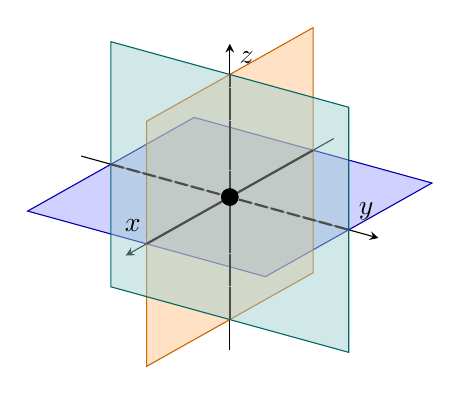
\begin{tikzpicture}
\begin{axis}[
    view={125}{25},
    axis lines=center,
    xlabel={$x$},
    ylabel={$y$},
    zlabel={$z$},
    xmin=-2.5, xmax=2.5,
    ymin=-2.5, ymax=2.5,
    zmin=-2.5, zmax=2.5,
    xtick=\empty, ytick=\empty, ztick=\empty,
    width=8cm, height=8cm,
    clip=false
]

% Plane 1: z = 0 (horizontal, blue)
\addplot3[
    surf,
    shader=flat,
    draw=blue!70!black,
    fill=blue!40,
    fill opacity=0.45,
    samples=2,
    domain=-2:2,
    y domain=-2:2
] {0};

% Plane 2: y = 0 (vertical, orange)
\addplot3[
    surf,
    shader=flat,
    draw=orange!80!black,
    fill=orange!50,
    fill opacity=0.45,
    samples=2,
    domain=-2:2,
    y domain=-2:2
] ({x}, {0}, {y});

% Plane 3: x = 0 (vertical, teal)
\addplot3[
    surf,
    shader=flat,
    draw=teal!80!black,
    fill=teal!40,
    fill opacity=0.45,
    samples=2,
    domain=-2:2,
    y domain=-2:2
] ({0}, {x}, {y});

% Pairwise intersection lines
\addplot3[domain=-2:2, samples=2, thick, dashed, black!70] ({x}, {0}, {0});
\addplot3[domain=-2:2, samples=2, thick, dashed, black!70] ({0}, {x}, {0});
\addplot3[domain=-2:2, samples=2, thick, dashed, black!70] ({0}, {0}, {x});

% Unique intersection point at (0,0,0)
\addplot3[only marks, mark=*, mark size=3pt, black] coordinates {(0,0,0)};

\end{axis}
\end{tikzpicture}
\end{document}
